\documentclass[12pt]{article}
\usepackage{verbatim}
\usepackage[dvips]{epsfig}
\usepackage{color}
\usepackage{url}
\usepackage[colorlinks=true]{hyperref}

\begin{document}

\section*{GENESIS: Documentation}

{\bf Related Documentation:}
% start: userdocs-tag-replace-items related-do-nothing
% end: userdocs-tag-replace-items related-do-nothing

\subsection*{Figure\,10}

\begin{figure}[h]
\centering
   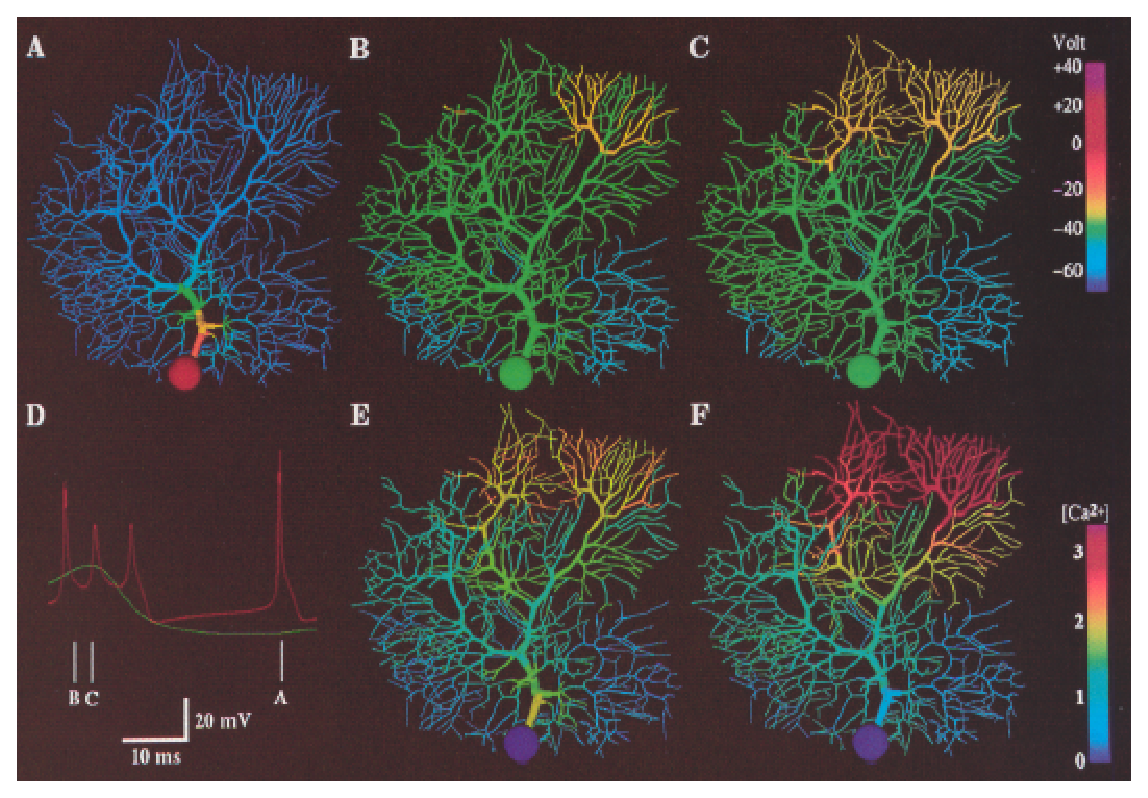
\includegraphics[scale=0.75]{figures/Fig.1.10.eps}
   \caption{False color representation of membrane potential and Ca$^{2+}$ concentration in the complete model during a 2.0\,nA current injection in the soma. {\it A}: Membrane potential distribution during a somatic action potential. {\it B}: Membrane potential distribution at the beginning of a dendritic spike. {\it C}: Membrane potential distribution 1.6\,ms later, when the dendritic spike had peaked. {\it D}: Somatic (red) and dendritic (green) recordings with the times when images A--C were taken indicated. {\it E}: Submembrane Ca$^{2+}$ concentration at same time as {\it B}. {\it F}: Submembrane Ca$^{2+}$ concentration at same time as {\it C}. Note the nonlinear voltage scale, which is expanded between -60 and -20\,mV.}
   \label{fig:DS1.10}
\end{figure}

\bibliographystyle{plain}
\bibliography{../tex/bib/g3-refs.bib}

\end{document}
